\documentclass[12pt]{beamer}

\mode<presentation>
\usetheme{metropolis}

\usepackage{appendixnumberbeamer}
\usepackage[brazil]{babel}
\usepackage{booktabs}
\usepackage[scale=2]{ccicons}
\usepackage{fontspec}
\usepackage{graphicx}

\setsansfont[BoldFont={Fira Sans SemiBold}]{Fira Sans Book}

\setbeamertemplate{frame footer}{\href{http://creativecommons.org/licenses/by-sa/4.0/}{\ccbysa}
                                 \footnotesize{ \url{https://github.com/ayharano/aio-exemplo}}}

\newcounter{contador}

\graphicspath{ {.} }


\title{\small{Usando \texttt{\href{https://docs.python.org/3/library/asyncio.html}{asyncio}} para
              reescrever processamento sem dependência em código concorrente}}
\author{\href{https://alexandre.harano.net.br/}{Alexandre Yukio Harano}}
\institute[NIC.br]
{\href{https://www.nic.br/}{Núcleo de Informação e Coordenação do Ponto BR (NIC.br)}\\
 harano@nic.br\\
 alexandre@harano.net.br\\
 \url{https://alexandre.harano.net.br/}}
\date{\scriptsize{\href{https://www.meetup.com/pt-BR/Grupy-SP/events/246561769/}{São Paulo, 18 de Janeiro de 2018}
 --
\href{https://www.meetup.com/pt-BR/Grupy-SP/}{Grupy-SP}}}



\begin{document}

\maketitle

\begin{frame}{Índice}
  \setbeamertemplate{section in toc}[sections numbered]
  \tableofcontents[hideallsubsections]
\end{frame}



\section{Motivação}

\begin{frame}[standout]
  \begin{overprint}
    \LARGE{\vspace{4cm}
           Python é lento\only<1-2>{.}\only<3>{?}}\\
    \onslide<2>{\small{\vspace{2cm}
                \begin{flushright}
                  \textbf{Why Python is Slow: Looking Under the Hood}\\
                  \vspace{0.25cm}
                  \tiny{\url{https://jakevdp.github.io/blog/2014/05/09/why-python-is-slow/}}
                \end{flushright}}}
  \end{overprint}
\end{frame}

\begin{frame}[fragile]{Tempos de Resposta}
  \scriptsize{
  \begin{table}
    \vspace{-0.5cm}
    \begin{tabular}{@{} lr @{}}
      \toprule
      Ação & Tempo de resposta (ns)\\
      \midrule
      execução de instrução típica & 1 ns\\
      recuperar de memória cache L1 & 0,5 ns\\
      errar predição condicional & 5 ns\\
      recuperar de memória cache L2 & 7 ns\\
      travar/destravar mutex & 25 ns\\
      recuperar de memória principal & 100 ns\\
      enviar 2K bytes via rede 1Gbps & 20 000 ns\\
      ler 1MB sequencialmente da memória & 250 000 ns\\
      recuperar de um novo local do disco (busca) & 8 000 000 ns\\
      ler 1MB sequencialmente do disco & 20 000 000 ns\\
      enviar um pacote dos EUA para a Europa e receber a resposta & 150 000 000 ns\\
      \bottomrule
    \end{tabular}
  \end{table}}
  \begin{flushright}
    \footnotesize{\vspace{-0.75cm}
                  \textbf{Fonte:} Teach Yourself Programming in Ten Years, por Peter Norvig\\
                  \url{http://norvig.com/21-days.html#answers}}
  \end{flushright}
\end{frame}



\section{Histórico}

\begin{frame}[fragile]{PEPs relacionadas}
  \begin{description}
    \item[PEP\ \ 380] \href{https://www.python.org/dev/peps/pep-0380/}{Syntax for Delegating to a Subgenerator} (3.3+)\\
    \item[PEP\ 3156] \href{https://www.python.org/dev/peps/pep-3156/}{Asynchronous IO Support Rebooted: the "asyncio" Module} (3.4+)\\
    \item[PEP\ \ 492] \href{https://www.python.org/dev/peps/pep-0492/}{Coroutines with \texttt{async} and \texttt{await} syntax} (3.5+)\\
    \item[PEP\ \ 525] \href{https://www.python.org/dev/peps/pep-0525/}{Asynchronous Generators} (3.6+)\\
    \item[PEP\ \ 530] \href{https://www.python.org/dev/peps/pep-0530/}{Asynchronous Comprehensions} (3.6+)\\
  \end{description}
\end{frame}

\begin{frame}[fragile]{\href{https://www.python.org/dev/peps/pep-0380/}{PEP 380} e \href{https://www.python.org/dev/peps/pep-0492/}{PEP 492}}
  \begin{table}
    \tiny{
    \begin{tabular}{ll}
      Python 3.4+ (\href{https://www.python.org/dev/peps/pep-0380/}{PEP 380}) & Python 3.5+ (\href{https://www.python.org/dev/peps/pep-0492/}{PEP 492})\\
      \midrule
      \verb|import asyncio| & \verb|import asyncio|\\
       & \\
      \textbf{\texttt{@asyncio.coroutine}} & \verb||\\
      \verb|def hello_world():| & \textbf{\texttt{async def}}\verb| hello_world():|\\
      \verb|    print("Hello World!")| & \verb|    print("Hello World!")|\\
       & \\
      \textbf{\texttt{@asyncio.coroutine}} & \verb||\\
      \verb|def main():| & \textbf{\texttt{async def}}\verb| main():|\\
      \verb|    |\textbf{\texttt{yield from}}\verb| hello_world()| & \verb|    |\textbf{\texttt{await}}\verb| hello_world()|\\
       & \\
      \verb|loop = asyncio.get_event_loop()| & \verb|loop = asyncio.get_event_loop()|\\
      \verb|loop.run_until_complete(main())| & \verb|loop.run_until_complete(main())|\\
      \verb|loop.close()| & \verb|loop.close()|\\
      \bottomrule
    \end{tabular}}
  \end{table}
  \begin{flushleft}
    \vspace{-0.25cm}
    \scriptsize{\textbf{Baseado em:}\\}
    \tiny{\textbf{Python 3.4} Hello World Coroutine\\
          \url{https://docs.python.org/3.4/library/asyncio-task.html#example-hello-world-coroutine}\\
          \textbf{Python 3.5} Hello World Coroutine\\
          \url{https://docs.python.org/3.5/library/asyncio-task.html#example-hello-world-coroutine}}
  \end{flushleft}
\end{frame}



\section{Mecanismos disponíveis}

\begin{frame}[fragile]{Mecanismos disponíveis}
  \small{
  \textbf{\texttt{\href{https://docs.python.org/3/library/asyncio-eventloop.html}{asyncio.AbstractEventLoop}}}

  Efetua o controle da concorrência das corrotinas.\\\vspace{0.25cm}

  \textbf{\texttt{\href{https://docs.python.org/3/library/asyncio-eventloop.html\#asyncio.AbstractEventLoop.run\_forever}{run\_forever()}}}

  Executa continuamente até \texttt{stop()} ser chamado.\\\vspace{0.25cm}

  \textbf{\texttt{\href{https://docs.python.org/3/library/asyncio-eventloop.html\#asyncio.AbstractEventLoop.run\_until\_complete}{run\_until\_complete(future)}}}

  Executa até \texttt{future} ser completado.\\\vspace{0.25cm}
  }
\end{frame}

\begin{frame}{Diagrama sobre corrotinas}
  \begin{center}
    \vspace{-0.5cm}
    \href{https://docs.python.org/3/library/asyncio-task.html\#example-chain-coroutines}{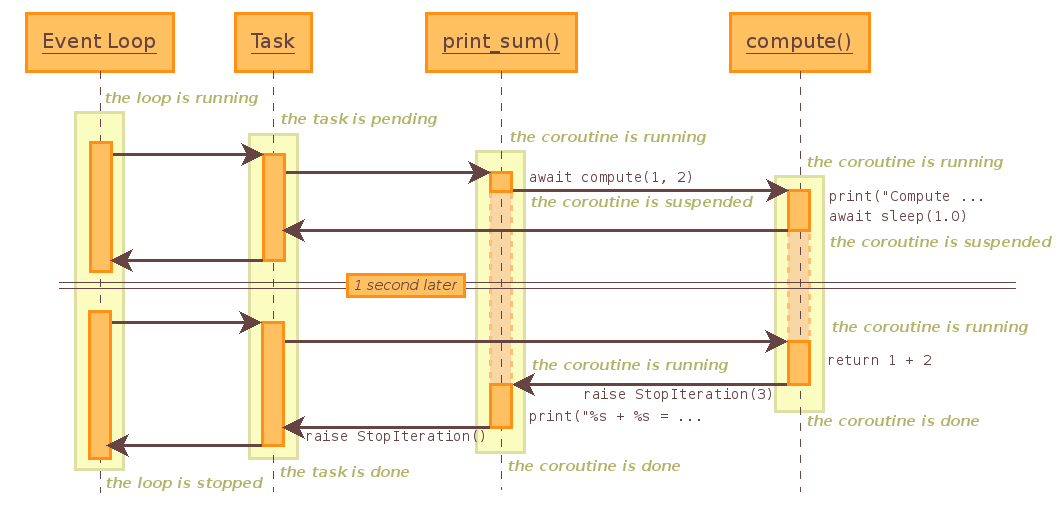
\includegraphics[width=11cm]{tulip_coro}}
  \end{center}
  \begin{flushleft}
    \footnotesize{\vspace{-0.5cm}
                  \textbf{Fonte:} Example: Chain coroutines\\
                  \tiny{\url{https://docs.python.org/3/library/asyncio-task.html\#example-chain-coroutines}}}
  \end{flushleft}
\end{frame}

\begin{frame}[fragile]{Mecanismos disponíveis}
  \small{
  \textbf{\texttt{\href{https://docs.python.org/3/library/asyncio-task.html\#asyncio.Future}{asyncio.Future}}}

  Permite a execução de corrotinas de forma não bloqueante: é usado para armazenar o resultado do cálculo efetuado dentro de uma corrotina quando passado por parâmetro. Pode disparar um \textit{callback} se configurado para tal, mas não é necessário.

  \textbf{\texttt{set\_result(valor)}} usado para armazenar um \texttt{valor}.\\

  \textbf{\texttt{result()}} usado para obter \texttt{valor} calculado dentro de uma corrotina. \emph{Só pode ser chamado depois que \texttt{valor} tiver sido atribuido!}
  }
\end{frame}

\begin{frame}[fragile]{Mecanismos disponíveis}
  \small{
  \textbf{\texttt{\href{https://docs.python.org/3/library/asyncio-task.html\#asyncio.ensure\_future}{asyncio.ensure\_future(coro\_or\_future, *, loop=None)}}}

  Agenda a execução de uma corrotina.\\\vspace{0.25cm}

  \textbf{\texttt{\href{https://docs.python.org/3/library/asyncio-task.html\#asyncio.shield}{asyncio.shield(arg, *, loop=None)}}}

  Protege a corrotina passada por parâmetro contra cancelamento da corrotina exterior.\\\vspace{0.25cm}

  \textbf{\texttt{\href{https://docs.python.org/3/library/asyncio-task.html\#asyncio.sleep}{asyncio.sleep(delay, result=None, *, loop=None)}}}

  Corrotina para esperar \texttt{delay} segundos.\\\vspace{0.25cm}
  }
\end{frame}

\begin{frame}[fragile]{Mecanismos disponíveis}
  \small{
  \textbf{\texttt{\href{https://docs.python.org/3/library/asyncio-task.html\#asyncio.gather}{asyncio.gather(*coros\_or\_futures, loop=None, return\_exceptions=False)}}}

  Agrega os resultados dos \texttt{asyncio.Future} passados por parâmetro de acordo com a ordem de instanciação da sequência original (não necessariamente a ordem de término).

  \textbf{\texttt{\href{https://docs.python.org/3/library/asyncio-task.html\#asyncio.wait\_for}{asyncio.wait\_for(fut, timeout, *, loop=None)}}}

  Espera \texttt{timeout} segundos: caso não termine no tempo, cancela \texttt{fut} e lança \texttt{asyncio.TimeoutError}.\\\vspace{0.25cm}
  }
\end{frame}

\begin{frame}[fragile]{Mecanismos disponíveis}
  \small{
  \textbf{\texttt{\href{https://docs.python.org/3/library/asyncio-task.html\#asyncio.wait}{asyncio.wait(futures, *, loop=None, timeout=None, return\_when=ALL\_COMPLETED)}}}

  Espera completar \texttt{asyncio.Future} e corrotinas passadas por parâmetro. A sequência do parâmetro \emph{não pode ser vazia}. São 3 condições de devoluções possíveis:

  \begin{description}\footnotesize{
    \item[\texttt{FIST\_COMPLETED}] assim que algum completar. 
    \item[\texttt{FIST\_EXCEPTION}] assim que a primeira \texttt{Exception} for lançada. Caso não tenha nenhuma, é equivalente a \texttt{ALL\_COMPLETED}. 
    \item[\texttt{ALL\_COMPLETED}] somente quando todos completarem. Opção \textit{default}.
  }\end{description}
  }
\end{frame}

\begin{frame}[fragile]{Mecanismos disponíveis}
  \small{
  \textbf{\texttt{\href{https://docs.python.org/3/library/asyncio-task.html\#asyncio.wait}{asyncio.wait(futures, *, loop=None, timeout=None, return\_when=ALL\_COMPLETED)}}}

  Uso:

  \verb+done, pending = await asyncio.wait(fs)+

  Entrega uma tupla de dois valores: \texttt{done, pending}.

  Não lança \texttt{asyncio.TimeoutError}: os não completos dentro de \texttt{timeout} são entregues dentro de \texttt{pending}.
  }
\end{frame}



\section{Exemplos de Uso}

\begin{frame}[fragile]{\texttt{\href{https://github.com/aio-libs}{aio-libs}}}
  \begin{table} 
    \vspace{-0.25cm}
    \begin{tabular}{rl}
      \textbf{Cliente/servidor \texttt{http}} & 
      \texttt{\href{https://github.com/aio-libs/aiohttp}{aiohttp}} \\
      & \\
      \textbf{Cliente/servidor \texttt{ftp}} &
      \texttt{\href{https://github.com/aio-libs/aioftp}{aioftp}} \\
      & \\
      \textbf{Banco de dados} &
      \texttt{\href{https://github.com/aio-libs/aiopg}{aiopg}} \\
      &
      \texttt{\href{https://github.com/aio-libs/aiomysql}{aiomysql}} \\
      & \\
      \textbf{Outros} &
      \texttt{\href{https://github.com/aio-libs/aioredis}{aioredis}} \\
      &
      \texttt{\href{https://github.com/aio-libs/aiodocker}{aiodocker}} \\
      &
      \texttt{...} \\
    \end{tabular}
  \end{table}
\end{frame}

\begin{frame}[fragile]{\texttt{\href{https://docs.python.org/3/library/asyncio.html}{asyncio}} boilerplate}
  \scriptsize{\vspace{-0.25cm}
              \begin{verbatim}#!/usr/bin/env python3
""" asyncio working boilerplate for Python 3.5+. """

import asyncio
import sys

async def main(argv, *args, **kwargs):
    return

if __name__ == '__main__':
    _LOOP = asyncio.get_event_loop()
    _LOOP.run_until_complete(main(sys.argv))
    _PENDING = asyncio.Task.all_tasks()
    _LOOP.run_until_complete(asyncio.gather(*_PENDING))
    _LOOP.stop()
    _LOOP.close()\end{verbatim}}
  \begin{flushright}
    \tiny{\vspace{-0.25cm}
          Disponível em \url{https://github.com/ayharano/aio-exemplo/blob/master/aio\_boilerplate.py}}
  \end{flushright}
\end{frame}

\begin{frame}[fragile]{Lista de tarefas pendentes}
  \footnotesize{\textbf{Propósito} Apresentar feedback visual via CLI\\
  \begin{enumerate}\scriptsize{
    \item Recebe \texttt{dict} que mapeia \texttt{asyncio.Future} para um rótulo.
    \item Inicializa contador em zero.
    \item Calcula \texttt{set} de instâncias de \texttt{asyncio.Future} pendentes.
    \item Inicializa \texttt{set} de esperas de \texttt{asyncio.sleep}.
    \setcounter{contador}{\value{enumi}}
  }\end{enumerate}}
\end{frame}

\begin{frame}[fragile]{Lista de tarefas pendentes}
  \begin{enumerate}
    \scriptsize{
    \setcounter{enumi}{\value{contador}}
    \item Enquanto existirem \texttt{asyncio.Future} pendentes:
      \begin{enumerate}\scriptsize{
        \item Chama \texttt{asyncio.sleep} e armazena no \texttt{set} de esperas.
        \item Chama \texttt{asyncio.wait} com a condição de \texttt{FIRST\_COMPLETED}.
        \item Analisa as instâncias de \texttt{asyncio.Future} completadas:
          \begin{itemize}\scriptsize{
            \item Se tiver \texttt{asyncio.Future} com rótulo, armazena o rótulo.
            \item Registra se a espera mais recente estiver completa.
          }\end{itemize}
        \item Apresenta todos os rotulados completados na ordem.
        \item Se tiver algum rotulado completo, zera o contador.\\
              Senão:
           \begin{itemize}\scriptsize{
            \item[] Se contador completou um ciclo, imprime todos os rótulos dos
                     \texttt{asyncio.Future} pendentes com quebra de linha e zera o contador.\\
                    Senão, incrementa o contador e imprime \texttt{'.'}.
          }\end{itemize}
        \item Atualiza \texttt{set} de \texttt{asyncio.Future} pendentes como interseção das rotuladas.
      }\end{enumerate}
  }\end{enumerate}
\end{frame}

\begin{frame}[fragile]{Exemplo de \texttt{\href{https://github.com/ayharano/aio-exemplo/blob/master/apresenta\_pend\%C3\%AAncias.py}{apresenta\_pendências.py}}}
  \tiny{\begin{verbatim}(aio-exemplo-kaFLRWdV) bash-3.2$ python3 apresenta_pendências.py
.................................................. [faltam A, B, C]
.................................................. [faltam A, B, C]
.................................................. [faltam A, B, C]
.................................................. [faltam A, B, C]
............ A completou!
.................................................. [faltam B, C]
.................................................. [faltam B, C]
...... B completou!
.................................................. [falta C]
.................................................. [falta C]
...... C completou!
!\end{verbatim}}
\end{frame}

\begin{frame}[fragile]{Estrutura usual de processamento}
  \textbf{Coleta}

  \textbf{Processamento}

  \textbf{Análise}

  \textbf{Apresentação}
\end{frame}

\begin{frame}[fragile]{Estatísticas de livros do Machado de Assis}
  \small{
  \textbf{Coleta} \\
  Extração da versão \texttt{txt} dos livros do Machado de Assis disponíveis no \href{http://www.gutenberg.org/}{Project Gutenberg}.

  \textbf{Processamento} \\
  Leitura dos arquivos para memória e extração das linhas de interesse de cada livro.

  \textbf{Análise} \\
  Análise das linhas de acordo com critérios arbitrários.

  \textbf{Apresentação} \\
  Apresentação de estatísticas coletadas ao usuário.
  }
\end{frame}

\begin{frame}[fragile]{\href{http://www.gutenberg.org/}{Project Gutenberg}}
    \href{http://www.gutenberg.org/}{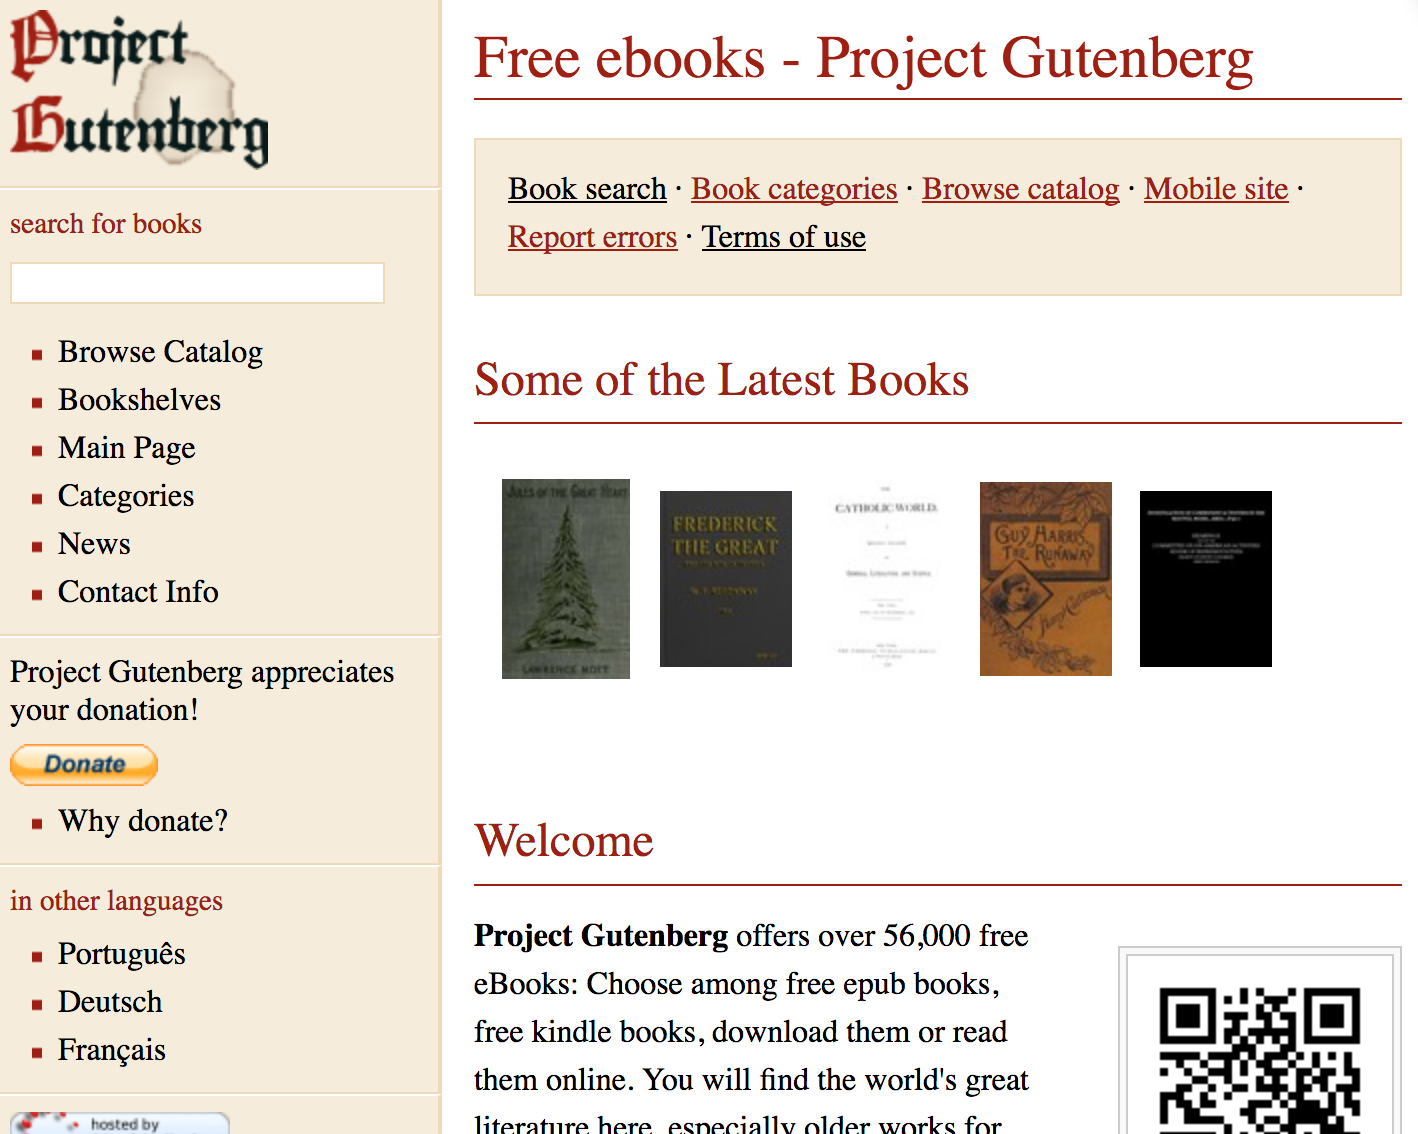
\includegraphics[width=9cm]{gutenberg_site}}
\end{frame}

\begin{frame}[fragile]{\href{http://www.gutenberg.org/}{Project Gutenberg}}
    \href{http://www.gutenberg.org/}{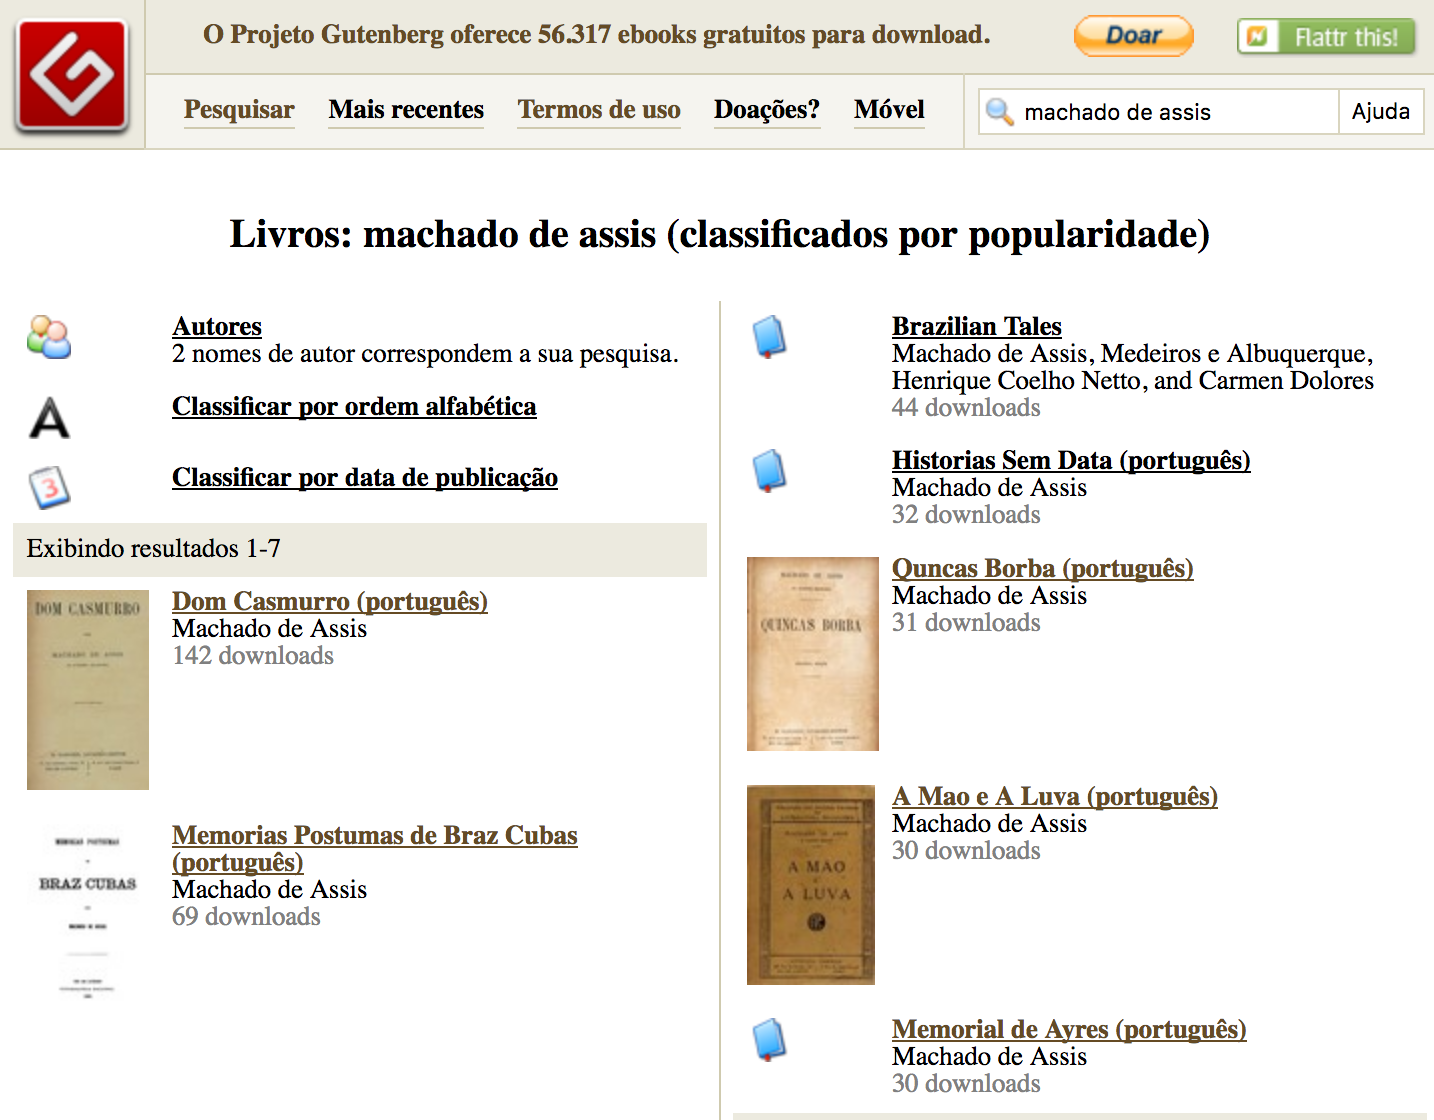
\includegraphics[width=9cm]{gutenberg_busca}}
\end{frame}

\begin{frame}[fragile]{\href{http://www.gutenberg.org/}{Project Gutenberg}}
    \href{http://www.gutenberg.org/}{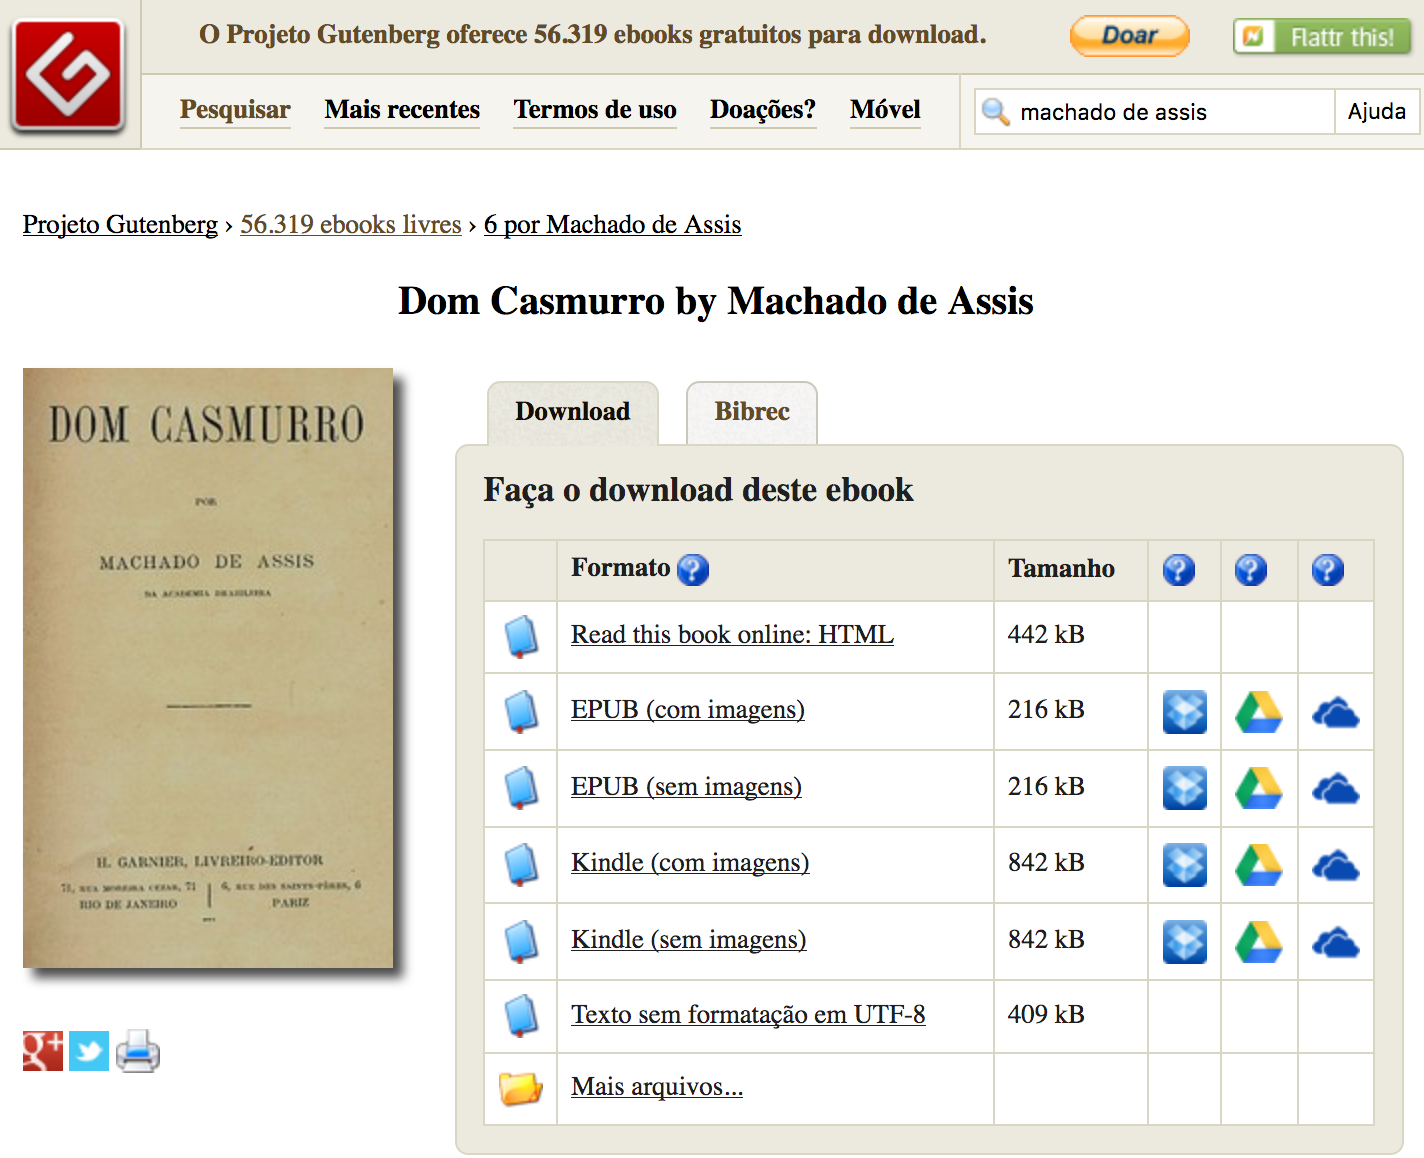
\includegraphics[width=9cm]{gutenberg_lista}}
\end{frame}

\begin{frame}[fragile]{\href{http://www.gutenberg.org/wiki/Gutenberg:Information\_About\_Robot\_Access\_to\_our\_Pages}{Information About Robot Access to our Pages}}
    \href{http://www.gutenberg.org/wiki/Gutenberg:Information\_About\_Robot\_Access\_to\_our\_Pages}{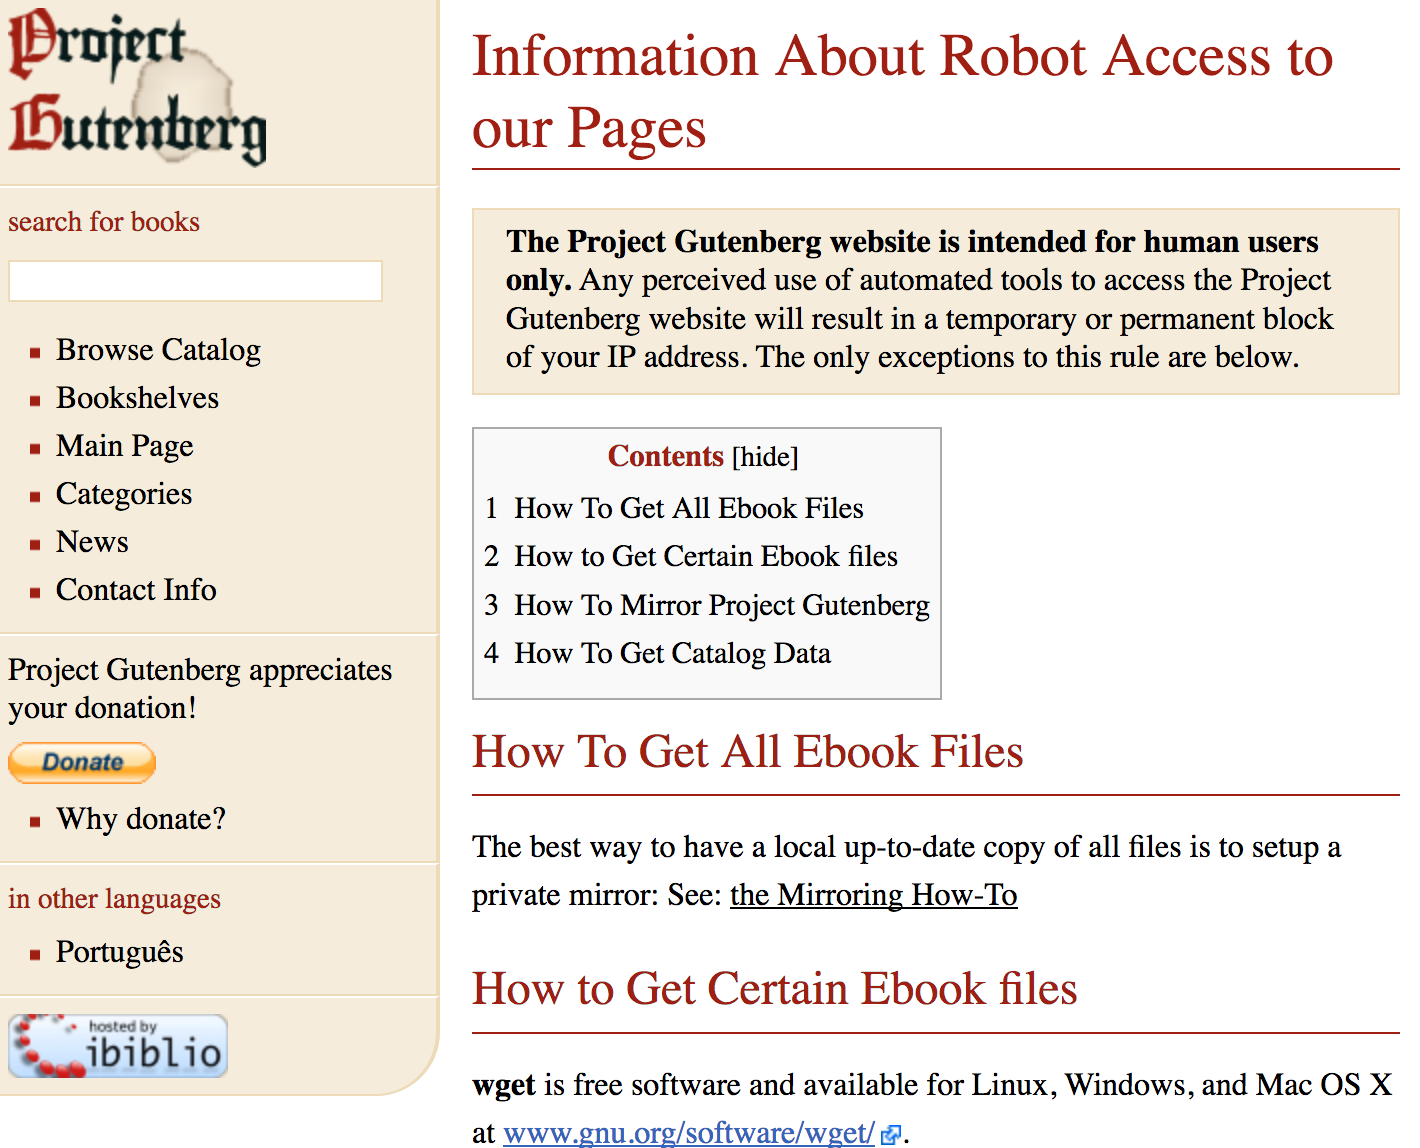
\includegraphics[width=9cm]{gutenberg_robot}}
\end{frame}

\begin{frame}[fragile]{\href{http://www.gutenberg.org/wiki/Gutenberg:Information\_About\_Robot\_Access\_to\_our\_Pages}{Information About Robot Access to our Pages}}

  Algumas regras sobre a coleta automatizada (pelo \href{http://www.gutenberg.org/wiki/Gutenberg:Terms\_of\_Use}{Termos de Uso} do \href{http://www.gutenberg.org/}{Project Gutenberg}, a partir de 100 livros por dia é considerado automatizado):

  \begin{itemize}
    \item Esperar 2 segundos entre as coletas;

    \item Usar mirrors para coletar os livros (deveríamos utilizar neste exemplo).
  \end{itemize}
\end{frame}

\begin{frame}[fragile]{Estatísticas de livros do Machado de Assis}
  Foram montadas 4 versões de módulos:

  \begin{itemize}
    \item Versão síncrona e assíncrona.
    \item Agrupada por etapa e agrupada por livro (afeta processamento e análise).
  \end{itemize}

  Funções de coleta, processamento por livro, análise por livro e apresentação foram reunidas por categoria de sincronicidade (\ \texttt{\_base\_estatísticas\_livro\_assíncrono.py} e \texttt{\_base\_estatísticas\_livro\_síncrono.py}\ )
\end{frame}

\begin{frame}[fragile]{Estatísticas de livros do Machado de Assis}
  \scriptsize{
  \begin{table}
    \vspace{-0.5cm}
    \begin{tabular}{@{} rcc @{}}
      \toprule
      Função & Módulos síncronos & Módulos assíncronos\\
      \midrule
      Cliente \texttt{http} & \texttt{requests} & \texttt{aiohttp}\\
      \midrule
      Manipulação de arquivos & \texttt{pathlib} & \texttt{aiofiles}\\
                              & \texttt{(stdlib)} & \\
      \bottomrule
    \end{tabular}
  \end{table}}

  Além disso, foi utilizado o \texttt{BeautifulSoup} para representação dos arquivos HTML.
\end{frame}

\begin{frame}[fragile]{Estatísticas de livros do Machado de Assis}
  Exemplo de apresentação de estatísticas de um livro:

  \tiny{\begin{verbatim}[ Estatísticas de 'Memorias Postumas de Braz Cubas' de 'Machado de Assis' ]

    Número de linhas sem nenhum caractere visível: 2232
    Número de linhas com caractere visível: 6208
    Total de linhas: 8440

    Número de caracteres visíveis: 300860
    Número de sequências contíguas de caracteres visíveis: 61549

    Caracter sensível a maiúsculas e minúsculas mais utilizado: 'a' (36332 vezes).
    Caracter insensível a maiúsculas e minúsculas mais utilizado: 'a' (36978 vezes).

    Sequência sensível a maiúsculas e minúsculas mais utilizada: 'a' (2360 vezes).
    Sequência insensível a maiúsculas e minúsculas mais utilizada: 'a' (2537 vezes).

    Maiores sequências sensíveis a maiúsculas e minúsculas:
    'Constantinopla,--modernas,--em', 'tremula,--coitadinha,--tremula' (30 caracteres).
    Maiores sequências insensíveis a maiúsculas e minúsculas
    'constantinopla,--modernas,--em', 'tremula,--coitadinha,--tremula' (30 caracteres).\end{verbatim}}
\end{frame}

\begin{frame}[fragile]{Estatísticas de livros do Machado de Assis}
  Análise via \texttt{\href{https://docs.python.org/3/library/profile.html}{cProfile}} e \texttt{\href{https://docs.python.org/3/library/profile.html}{pstats}}

  \footnotesize{\textbf{\texttt{Condição}} \\
  \scriptsize{Arquivos dos livros já foram previamente coletados em execução anterior.}}

  \scriptsize{
  \begin{table}
    \vspace{-0.5cm}
    \begin{tabular}{@{} rrr @{}}
      \toprule
      Módulo & Tempo (s) & Chamadas de função \\
      \midrule
      estatísticas\_livro\_síncrono\_agrupado\_por\_etapa   & 4,995 &  6854857 \\
      estatísticas\_livro\_síncrono\_agrupado\_por\_livro   & 5,329 &  6854846 \\
      estatísticas\_livro\_assíncrono\_agrupado\_por\_etapa & 9,406 & 12267885 \\
      estatísticas\_livro\_assíncrono\_agrupado\_por\_livro & 9,030 & 12268402 \\
      \bottomrule
    \end{tabular}
  \end{table}}

  Observação: exemplo de uso de \texttt{\href{https://docs.python.org/3/library/profile.html}{cProfile}} e \texttt{\href{https://docs.python.org/3/library/profile.html}{pstats}} em \\
  \tiny{\url{http://stefaanlippens.net/python\_profiling\_with\_pstats\_interactive\_mode/}}
\end{frame}

\begin{frame}[fragile]{Estatísticas de livros do Machado de Assis}
  Por que as versões assíncronas foram piores nesse caso?

  \begin{itemize}\small{
    \item Os livros já estavam coletados.
    \item Mesmo nas versões assíncronas, as regras de robôs foram respeitadas, então a coleta é sequencial.
    \item Uma vez que os livros estejam em memória, nesse caso, o uso de \texttt{for} sequencial é mais vantajoso, pois são menos chamadas de função (instanciação de \texttt{asyncio.Future} e \texttt{asyncio.ensure\_future}).
    \item Caso estivesse projetado o uso de outros recursos de I/O externo (disco, BD, rede, etc), o resultado poderia seria outro.
  }\end{itemize}
\end{frame}



\begin{frame}[standout]
  \LARGE{Obrigado!}
  \begin{block}{}
    \begin{flushright}
      \large{\href{https://alexandre.harano.net.br/}{Alexandre Yukio Harano}} \\ \vspace{0.25cm}
      \small{\href{mailto:harano@nic.br}{harano@nic.br}} \\ \vspace{0.25cm}
      \small{\href{mailto:alexandre@harano.net.br}{alexandre@harano.net.br}} \\
      \small{\url{https://alexandre.harano.net.br/}}
    \end{flushright}
  \end{block}
\end{frame}



\appendix

\begin{frame}[allowframebreaks]
  \frametitle<presentation>{Referências}
  {
    \bibliographystyle{plainnat}
    \bibliography{20180118_grupy_sp_aio_exemplo}
    \nocite{PEP380}
    \nocite{PEP3156}
    \nocite{asyncio}
    \nocite{PEP492}
    \nocite{PEP525}
    \nocite{PEP530}
    \nocite{VanderPlasJake14}
    \nocite{RamalhoLuciano15}
    \nocite{CannonBrett16}
    \nocite{Langa16}
    \nocite{FDLaura17}
  }
\end{frame}

\end{document}
